\documentclass{article}

\usepackage{fancyhdr}
\usepackage{extramarks}
\usepackage{amsmath}
\usepackage{amsthm}
\usepackage{amsfonts}
\usepackage{tikz}
\usepackage[plain]{algorithm}

\usetikzlibrary{automata,positioning}
\usepackage{titling}
\usepackage{chngcntr}
\counterwithin{figure}{section}
\usepackage{sectsty}
\sectionfont{\fontsize{15}{15}\selectfont}
\usepackage{multirow}
\usepackage{booktabs}
\usepackage{arydshln}
\usepackage[font={scriptsize}]{caption}
\usepackage{listings}
\usepackage{color}
\definecolor{mygreen}{RGB}{28,172,0} 
\definecolor{mylilas}{RGB}{170,55,241}
%
% Basic Document Settings
%

\topmargin=-0.45in
\evensidemargin=0in
\oddsidemargin=0in
\textwidth=6.5in
\textheight=9.0in
\headsep=0.25in

\linespread{1.1}

\pagestyle{fancy}
\lhead{\hmwkClass}
\rhead{\hmwkTitle}
\cfoot{\thepage}

\renewcommand\headrulewidth{0.4pt}
\renewcommand\footrulewidth{0.4pt}
\renewcommand{\thesubsubsection}{\alph{subsubsection})}
\setlength\parindent{0pt}

\lstdefinestyle{matlab}{
	language=Matlab,%
    basicstyle=\scriptsize,
    breaklines=true,%
    morekeywords={matlab2tikz},
    keywordstyle=\color{blue},%
    morekeywords=[2]{1}, keywordstyle=[2]{\color{black}},
    identifierstyle=\color{black},%
    stringstyle=\color{mylilas},
    commentstyle=\color{mygreen},%
    showstringspaces=false,%without this there will be a symbol in the places where there is a space
    %numbers=left,%
    %numberstyle={\tiny \color{black}},% size of the numbers
    %numbersep=9pt, % this defines how far the numbers are from the text
    emph=[1]{for,end,break},emphstyle=[1]\color{red}, %some words to emphasise
    %emph=[2]{word1,word2}, emphstyle=[2]{style},    
}
%
% Homework Details
%   - Title
%   - Due date
%   - Class
%   - Section/Time
%   - Instructor
%   - Author
%

\newcommand{\hmwkTitle}{}
\newcommand{\hmwkDueDate}{}
\newcommand{\hmwkClass}{Control of a Type-(1,1) Robot using Lyapunov Function}
\newcommand{\hmwkClassTime}{}
\newcommand{\hmwkClassInstructor}{}
\newcommand{\hmwkAuthorName}{}
\newcommand{\hmwkAuthorEmail}{Subodh.Mishra.eleves@ec-nantes.fr}
\newcommand{\figurescaling}{width=\textwidth}


\begin{document}
\clearpage
\thispagestyle{empty}
\clearpage
\noindent\rule{\textwidth}{0.4pt} \\
\textbf{\MakeUppercase{\hmwkClass}} \\
\textbf{\MakeUppercase{\hmwkTitle}} \\
\hmwkDueDate \\
%-----------------------------------TOP PAGE-----------------------------

\noindent\rule{\textwidth}{0.4pt}
\section{Introduction}
A simplified figure of the type (1,1) wheeled mobile robot is presented below in Figure 1.1. $a$ is the distance between the wheel centre of the fixed wheels and the centre of steerable wheel. $\beta$ is the steering angle and $\theta$ is the orientation of the $R_m$ frame (also called the robot frame) with respect to the $R_O$ frame(the world frame). The objective is to design a controller based on a Lyapunov function to make the robot follow a circular trajectory of radius 2 metre and angular velocity 0.5 radian per second. In Figure 1.1, $R$ is the perpendicular distance of the instantaneous centre of rotation (ICR) from the centre (s) of the steerable wheel.
\begin{figure}[H]
\centering
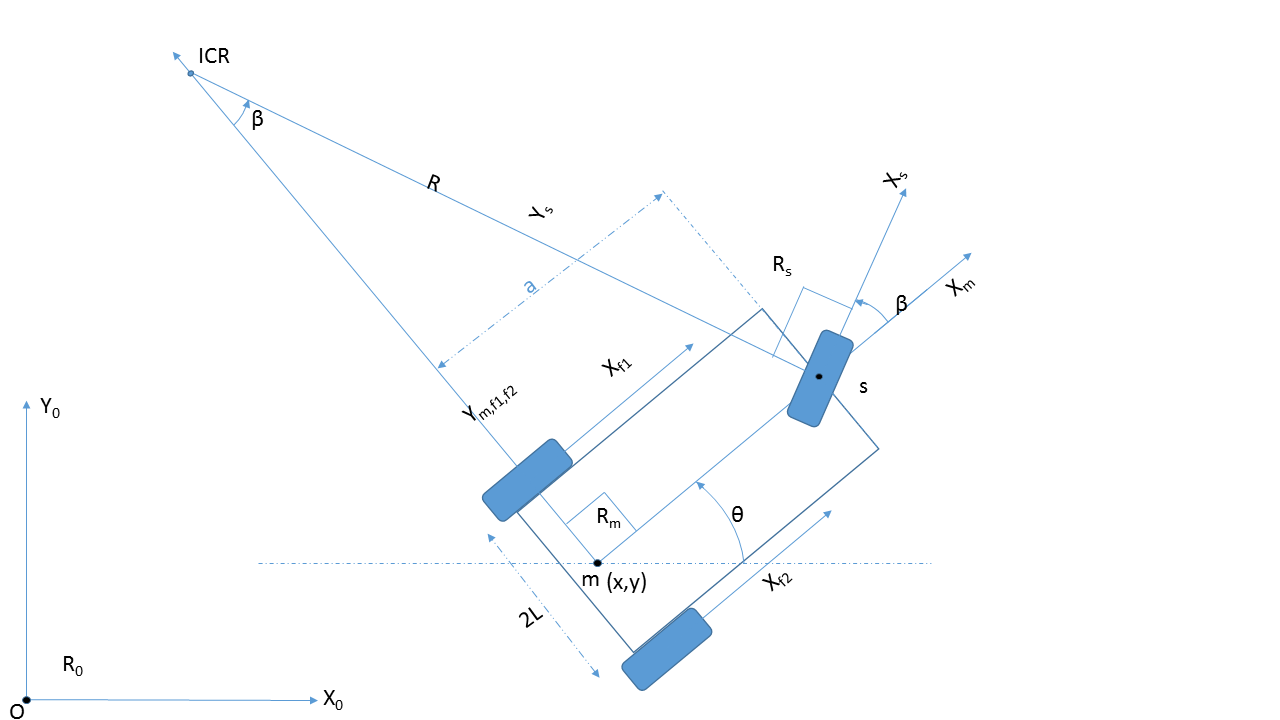
\includegraphics[width = 0.8\textwidth]{Figures/figure1.png}
\caption{Schematic of Type 11 Robot}
\label{fig:figure1}
\end{figure}
\section{The Posture Kinematic Model}
A possible kernel obtained from the matrix form of the no-skidding constraints for the type (1,1) wheeled mobile robot is:

\[\Sigma=
\begin{bmatrix}
    a\cos \beta \\
    0\\
    \sin \beta \\
\end{bmatrix}\]
Using the aforementioned kernel, the posture kinematic model of the type (1,1) robot is as follows:
\begin{align*} 
\dot{x}&=a\cos \theta \cos \beta u_m\\ 
\dot{y}&=a\sin \theta \cos \beta u_m\\
\dot{\theta}&= \sin \beta u_m\\
\dot{\beta}&=u_s
\end{align*}
Here, $u_m$ and $u_s$ are the inputs to the Posture Kinematic Model. While $u_s$ is the rate of change of orientation of the steering wheel, $u_m$ is \textbf{not} the net translational velocity of the robot.  
\section{Configuration Kinematic Model and Wheel Motorization}
For the same kernel as discussed in the previous section, the complete Configuration Kinematic Model of the type (1,1) wheeled mobile robot is:

\[\begin{bmatrix}
\dot{x}\\
\dot{y}\\
\dot{\theta}\\
\dot{\beta}\\
\dot{\phi}_{f1}\\
\dot{\phi}_{f2}\\
\dot{\phi}_{s}\end{bmatrix}=\begin{bmatrix}
 a\cos \beta \cos \theta & 0\\
 a\cos \beta \sin \theta & 0\\
 \sin \beta & 0\\
 0 & 1\\
 \frac{L\sin \beta + a \cos \beta}{r} & 0\\
 -\frac{L\sin \beta - a \cos \beta}{r} & 0\\
 \frac{a}{r} & 0\end{bmatrix} \begin{bmatrix}
 u_m \\ u_s
 \end{bmatrix}\]
 Here $\dot{\phi}_{f1}$, $\dot{\phi}_{f2}$ and $\dot{\phi}_{s}$ are the angular velocities of the fixed wheels and the steerable wheel about their corresponding spin axes and $2L$ is the distance between the two fixed wheels(the origin of the robot frame,$R_m$, is at the centre of the common axle of the two fixed wheels).
 \subsection{Wheel Motorisation}
 The degree of mobility of the type (1,1) wheeled mobile robot is $\delta m=$ 1. Hence, only 1 out of the last three rows of the configuration kinematic models needs to be picked to complete the motorisation of this robot. Owing to mathematical simplicity and ease of inversion, the last row is chosen, which implies the spin of the steerable wheel about its y-axis is motorized. It should be noted that the steering joint (joint angle $\beta$), which gives the rotation of the steerable wheel about its z-axis, is also motorized, but this does not come under wheel motorisation. The wheel motorisation obtained is:
 $$\dot{\phi}_s=\frac{a}{r}u_m$$
The above equation is the inverse kinematic model.
\section{Theoritical study}
For tracking, the point $s$ is used. Point $s$ is the origin of the steerable wheel frame($R_s$,refer Figure 1.1). The orientation of this frame with respect to the 
$R_0$ frame is $\theta+\beta$. A new variable $\psi$ is defined, where $\psi=\theta+\beta$. In the frame $R_0$, the posture to be tracked is:

\begin{align*} 
x_{s}&=x+a\cos \theta\\ 
y_{s}&=y+a\sin \theta\\
\psi&=\theta + \beta
\end{align*}

Here, (x,y) is the coordinate of the point $m$ in the $R_0$ frame. On taking the time derivative of the equations above, the following equation are obtained:\\
\begin{align*} 
\dot{x}_{s}&=\dot{x}-a\dot{\theta}\sin \theta \\ 
\dot{y}_{s}&=\dot{y}+a\dot{\theta}\cos \theta \\
\dot{\psi}&=\dot{\theta} + \dot{\beta}
\end{align*}
Using the the posture kinematic model of section 2, the above equations can be written as:\\
\begin{align*} 
\dot{x}_{s}&=a\cos \theta \cos \beta u_m - a\sin \theta \sin \beta u_m=a\cos(\theta+\beta) u_m=a\cos \psi u_m\\ 
\dot{y}_{s}&=a\sin \theta \cos \beta u_m+a\cos \theta \sin \beta u_m=a\sin(\theta+\beta) u_m=a\sin \psi u_m\\
\dot{\psi}&=\sin \beta u_m+ u_s
\end{align*}

$\implies$

\[\begin{bmatrix}
^{0}\dot{x}_{s}\\
^{0}\dot{y}_{s}\\
\dot{\psi}\end{bmatrix}=\begin{bmatrix}
a\cos \psi & 0\\
a\sin \psi & 0\\
\sin \beta & 1
 \end{bmatrix} \begin{bmatrix} u_m \\ u_s \end{bmatrix} \]
 
 This is the rate of change of state variables of the actual robot. Similarly, the virtual robot (the reference), which needs to be tracked (or followed) can be described by the following equations:
 
 \[\begin{bmatrix}
^{0}\dot{x}_{sr}\\
^{0}\dot{y}_{sr}\\
\dot{\psi}_{r}\end{bmatrix}=\begin{bmatrix}
a\cos \psi_{r} & 0\\
a\sin \psi_{r} & 0\\
\sin \beta_{r} & 1
 \end{bmatrix} \begin{bmatrix} u_{mr} \\ u_{sr} \end{bmatrix} \]
 
All the state space equations developed above are with respect to the frame $R_0$.

Let error be defined as: $error=reference-actual$. In the $R_s$ frame, the errors in rate of change of $x$,$y$ and $\psi$ is:

\[\begin{bmatrix}
^{s}\dot{x}_{e}\\
^{s}\dot{y}_{e}\\
 \dot{\psi}_{e}\end{bmatrix}=\begin{bmatrix}
0\\
0\\
-\dot{\psi}
 \end{bmatrix} \times \begin{bmatrix} ^{s}x_{e}\\^{s}y_{e}\\\psi \end{bmatrix} + ^{s}\Omega_{0} (\psi)  \left[\begin{bmatrix} ^{0}\dot{x}_{sr}\\^{0}\dot{y}_{sr}\\ \dot{\psi}_{r} \end{bmatrix}-\begin{bmatrix} ^{0}\dot{x}_{s}\\^{0}\dot{y}_{s}\\ \dot{\psi} \end{bmatrix}\right]  \] 
 
Here, \[\Omega(\psi)=\begin{bmatrix}
\cos \psi & \sin \psi & 0\\
-\sin \psi & \cos \psi & 0\\
0&0&1 
\end{bmatrix}\] 
Using the equations developed in this section, the error model is simplified as:\\
\[\begin{bmatrix}
^{s}\dot{x}_{e}\\
^{s}\dot{y}_{e}\\
 \dot{\psi}_{e}\end{bmatrix}=\begin{bmatrix}
au_{mr} \cos \psi_{e}\\
au_{mr} \sin \psi_{e}\\
 u_{mr}\sin \beta_{r} + u_{sr}
 \end{bmatrix}  +  \begin{bmatrix} ^{s}y_{e}\sin \beta -a & ^{s}y_{e}\\
                                  -^{s}x_{e}\sin \beta    &-^{s}x_{e}\\
                                     -\sin \beta & -1\end{bmatrix} \begin{bmatrix} u_{m} \\ u_{s} \end{bmatrix}  \] 
 
In short, the error model can be written as:
$\dot{X}=f(X,\textbf{u})$
Here, $X$ is the state variable vector and $\textbf{u}$ is the control input vector.
Consider a Lyapunov function $V(X)$ for the system $\dot{X}=f(X,\textbf{u})$. Designing a Lyapunov controller means finding a control input vector $\textbf{u}$ to satisfy:\\
$$\dot{V}(X)=\frac{\partial V}{\partial X}\dot{X}=\frac{\partial V}{\partial X}f(X,\textbf{u})<0$$
The Lyapunov function chosen must be positive definite. For this system, the Lyapunov function chosen is:
$$V(X)=\frac{1}{2}(^{s}x_{e}^{2}+^{s}y_{e}^{2}+\frac{^{s}\psi_{e}^{2}}{K_y})$$
\\It can be guaranteed that this is a Lyapunov function because it is positive definite and clearly has continous partial derivatives.\\
$$\dot{V}(X)=\frac{\partial V}{\partial X}\dot{X}=\frac{\partial V}{\partial X}f(X,\textbf{u})<0$$
$\implies$
\[\begin{bmatrix}^{s}x_{e}&^{s}y_{e}&\frac{\psi_e}{K_y}\end{bmatrix}\begin{bmatrix}
^{s}\dot{x}_{e}\\
^{s}\dot{y}_{e}\\
 \dot{\psi}_{e}\end{bmatrix}<0\] 
 On simplifying:
 $$(au_{mr}\cos \psi_{e}-au_{mr})^{s}x_{e}+(\frac{au_{mr}\sin \psi_{e} ^{s}y_{e}}{\psi_{e}}+\frac{u_{mr}\sin \beta_{r}+u_{sr}}{K_y}-\frac{u_{mr}\sin \beta +u_{sr}}{K_y})\psi_{e}<0$$
 
 This inequality is satisfied if:
  \begin{align}
au_{mr}\cos\psi_{e}-au_{mr}&=-K_{x} ^sx_{e}\\
\frac{au_{mr}\sin \psi_{e} ^{s}y_{e}}{\psi_{e}}+\frac{u_{mr}\sin \beta_{r}+u_{sr}}{K_y}-\frac{u_{mr}\sin \beta +u_{sr}}{K_y}&=-\frac{K_{\psi}}{K_{y}}^{s}\psi_{e}
 \end{align}
 $\implies$
 \begin{align}
u_{m}&=\frac{au_{mr}\cos \psi_{e}+K_x ^{s}x_e}{a}\\
u_{s}&=K_{y}\frac{au_{mr}\sin \psi_e ^sy_e}{\psi_e}+K_{\psi}\psi_{e}+u_{mr}\sin\beta_{r}+u_{sr}-u_{mr}\sin \beta 
 \end{align}
The above equations yield the value of the control inputs.\\
Hence,
\[\textbf{u}=\begin{bmatrix}
\frac{au_{mr}\cos \psi_{e}+K_x ^{s}x_e}{a}\\
\frac{K_{y}au_{mr}\sin \psi_e ^sy_e}{\psi_e}+K_{\psi}\psi_{e}+u_{mr}\sin\beta_{r}+u_{sr}-u_{mr}\sin \beta 
 \end{bmatrix} \] 
The use of this control law makes the system globally asymptotically stable because the substitution of these values in $\dot{V}(x)$ yields:\\
$$\dot{V}(x)=-K_{x}^{s}x_{e}^2-K_{\psi}\frac{\psi_{e}^2}{K_{y}}$$\\
Choice of positive gains ensures $\dot{V}<0$ globally, hence the stability.\\
As can be seen in the equations 3 and 4, the knowledge of reference steering angle $\beta_r$, the reference steering angular velocity $u_{s}$ and the reference translational velocity of the steering wheel $u_{m}$ is required.\\
The control objective is to force the robot to move along a circular trajectory centred at $(0,0)$ with radius $R=2$ m and angular velocity of $\omega_{d}=0.5$ rad/s, this implies that the tangential velocity of the robot must be $1$ m/s.\\
Since the robot is expected to follow a circular trajectory, the reference steering angle must be a constant. From Figure 1.1 it can be concluded that for a circular path, the constant reference steering angle is: $$\beta_r=\sin^{-1}\frac{a}{R}$$
The translational velocity of the type (1,1) robot is $\dot{x}^{2}+\dot{y}^2=au_{m}cos \beta$ must be equal to the tangential velocity required to satisfy the control objective. If the tangential velocity is $V_{tangential}$ then:
$$\dot{x}^{2}+\dot{y}^2=au_{m}cos \beta=V_{tangential}$$
$\implies$
$$u_{m}=\frac{V_{tangential}}{a\cos\beta}$$ 

For the control objective specified, $V_{tangential}=R\omega_{d}=1$ m/s.
\section{Modelling}
\begin{figure}[H]
\centering
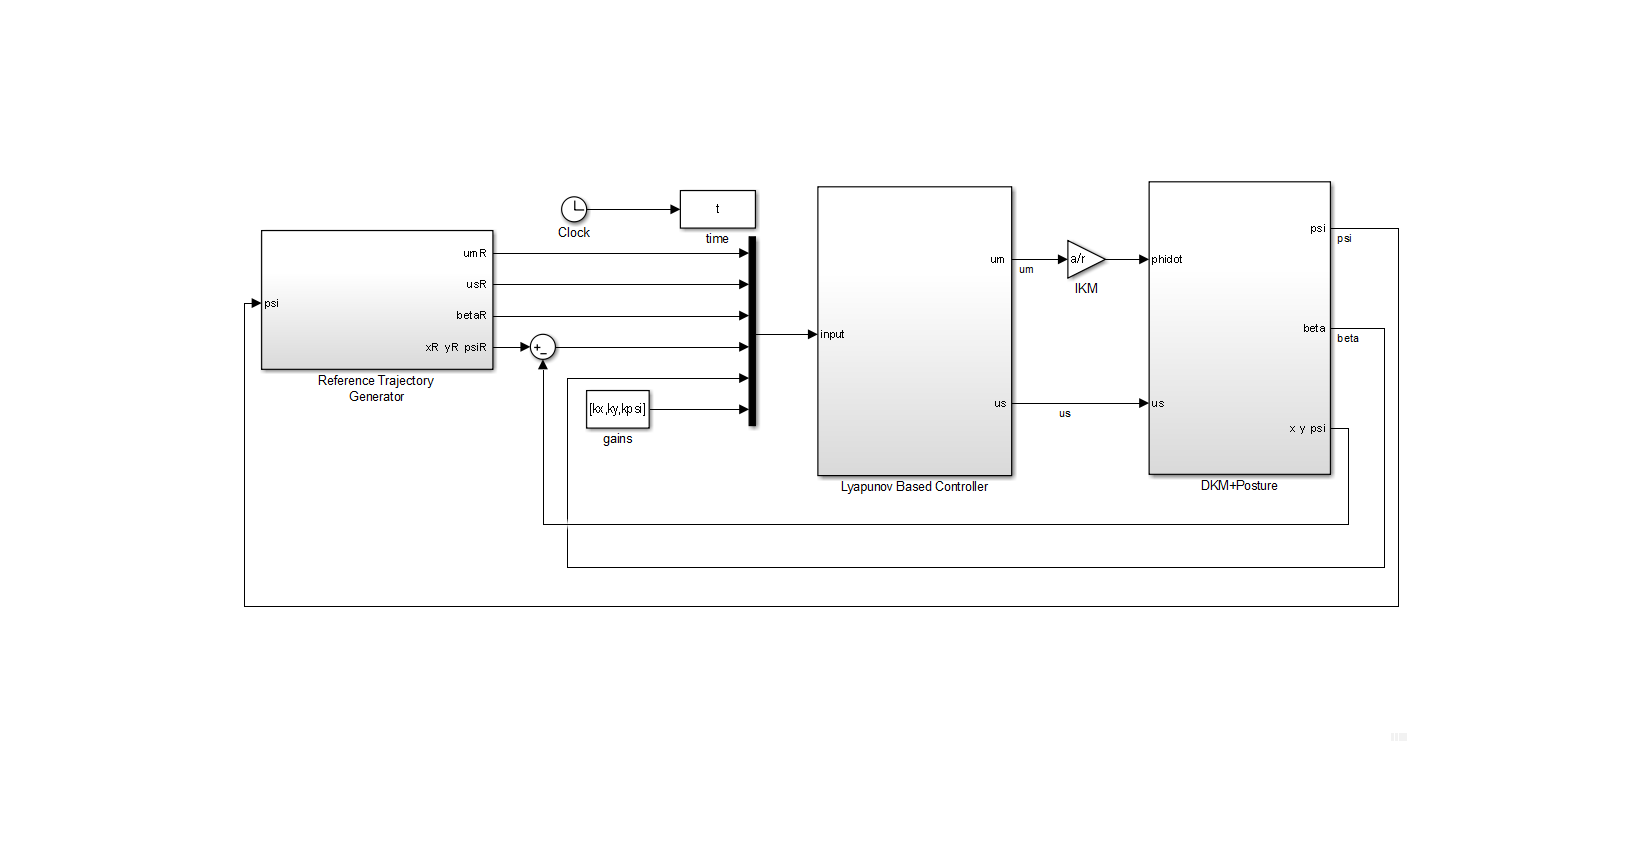
\includegraphics[width = 0.8\textwidth]{Figures/figure2.png}
\caption{Simulink model of a Lyapunov function  controlled Type(1,1) robot}
\label{fig:figure2}
\end{figure}
Figure 5.1 presents the \texttt{simulink} model of the Lyapunov function controlled Type(1,1) robot. A brief description of all the subsystems is presented below:\\

\begin{itemize}
\item The \texttt{Reference Trajectory Generator} subsystem generates the desired trajectory, in the $R_s$ frame, that the robot is expected to follow. Besides these, it also generates the reference steering wheel translational velocity $u_{mr}$, the reference steering wheel angular velocity $u_{sr}$ and the reference steering angle $\beta_{r}$.
\item The \texttt{Lyapunov Based Controller} subsystem implements the Lyapunov control law deduced in the previous section. It takes the errors in position (expressed in $R_s$ frame) \& orientations , $u_{mr}$, $u_{sr}$, $\beta_{r}$, $\beta$ and the controller gains as inputs and gives $\textbf{u}=[u_m,u_s]^T$ as the output.
\item The \texttt{DKM+Posture} block takes as input the steering wheel spin velocity $\dot{\phi}$ and the the steering angular velocity  $u_s$ as input. The subsytem implements the direct kinematic model and the posture kinematic model for the type (1,1) robot. There is a \texttt{Localisation} block inside this subsytem which shifts the tracking point to point s. Then a frame transformation is performed and the subsytem outputs the posture of the robot in the $R_s$ frame.
\end{itemize} 

\begin{figure}[H]
\centering
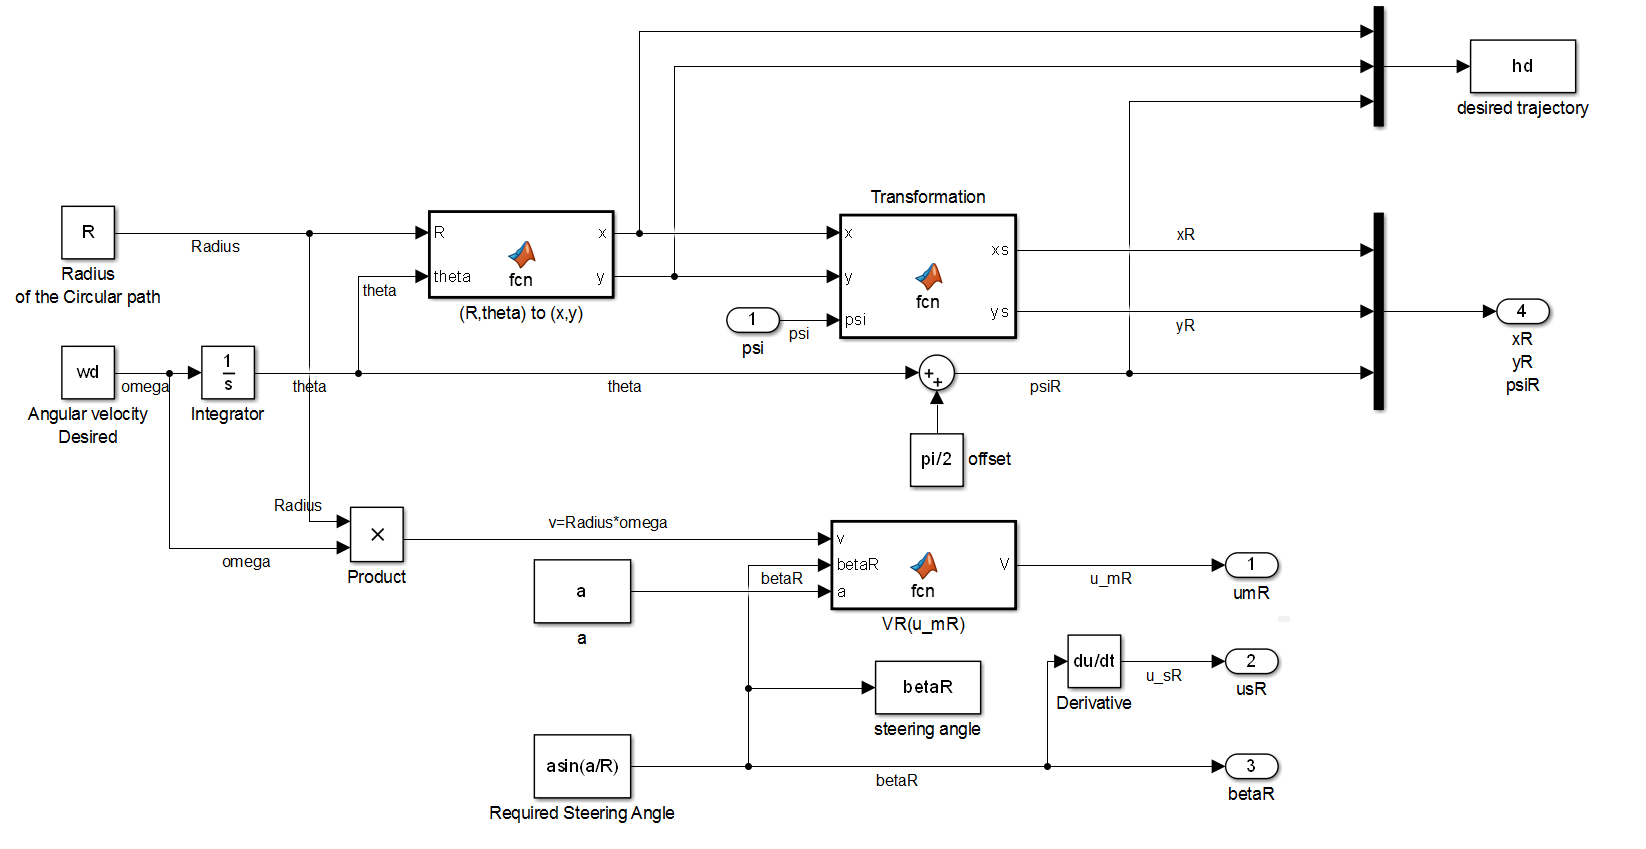
\includegraphics[width = 0.8\textwidth]{Figures/figure3.png}
\caption{Reference Trajectory Generator subsystem}
\label{fig:figure3}
\end{figure}

\begin{figure}[H]
\centering
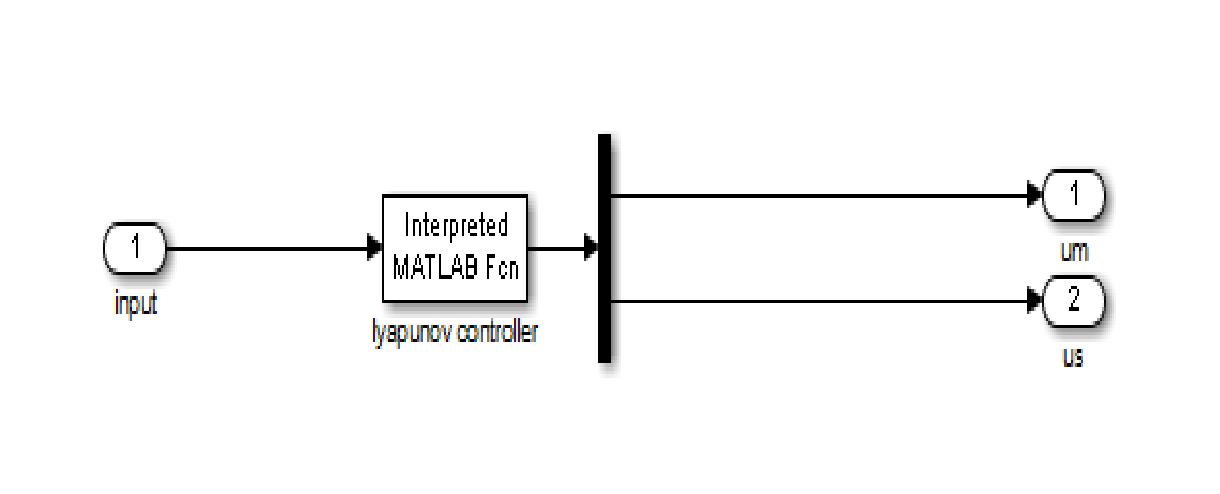
\includegraphics[width = 0.8\textwidth]{Figures/figure4.png}
\caption{Lyapunov Based Controller subsystem}
\label{fig:figure4}
\end{figure}

\begin{figure}[H]
\centering
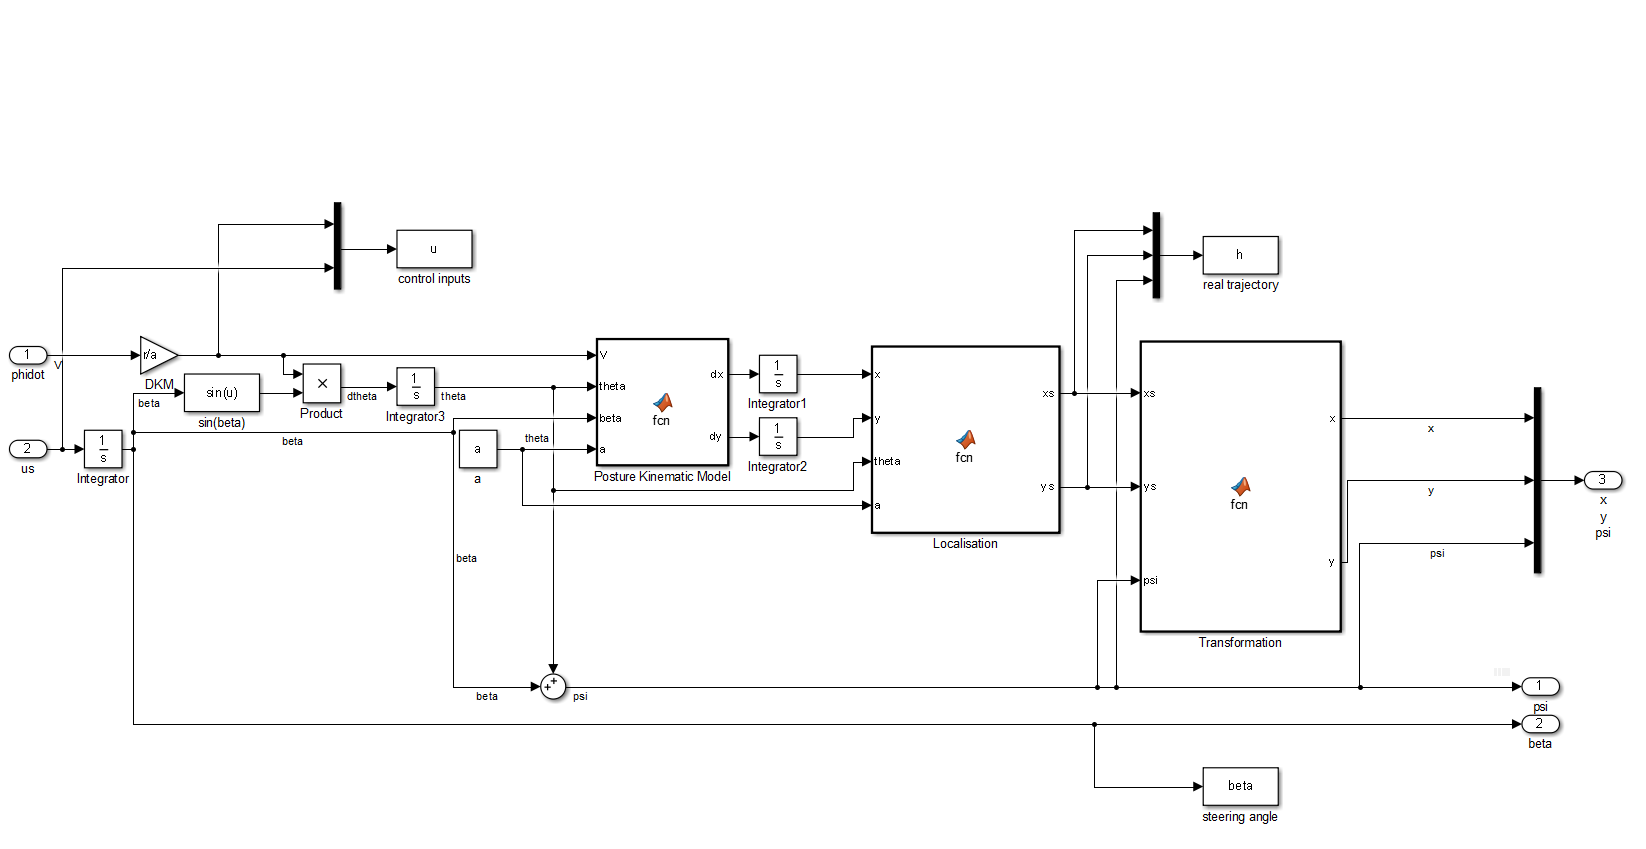
\includegraphics[width = 0.8\textwidth]{Figures/figure5.png}
\caption{DKM+Posture subsystem}
\label{fig:figure5}
\end{figure}

\subsection{Validation and Simulation}

\textbf{Remark:}The \texttt{fixed step ode4 Runge Kutta} solver is used with a time step of 0.001 second.\\
\textbf{Tuning: $K_{x}$,$K_{y}$ and $K_{\theta}$}\\
To ensure $\dot{V}<0$, $K_{x}$,$K_{y}$ and $K_{\theta}$ must all be positive.
\begin{itemize}
\item Tuning with $K_{x}=1$, $K_{y}=1$ and $K_{\theta}=1$: 
\begin{figure}[H]
\centering
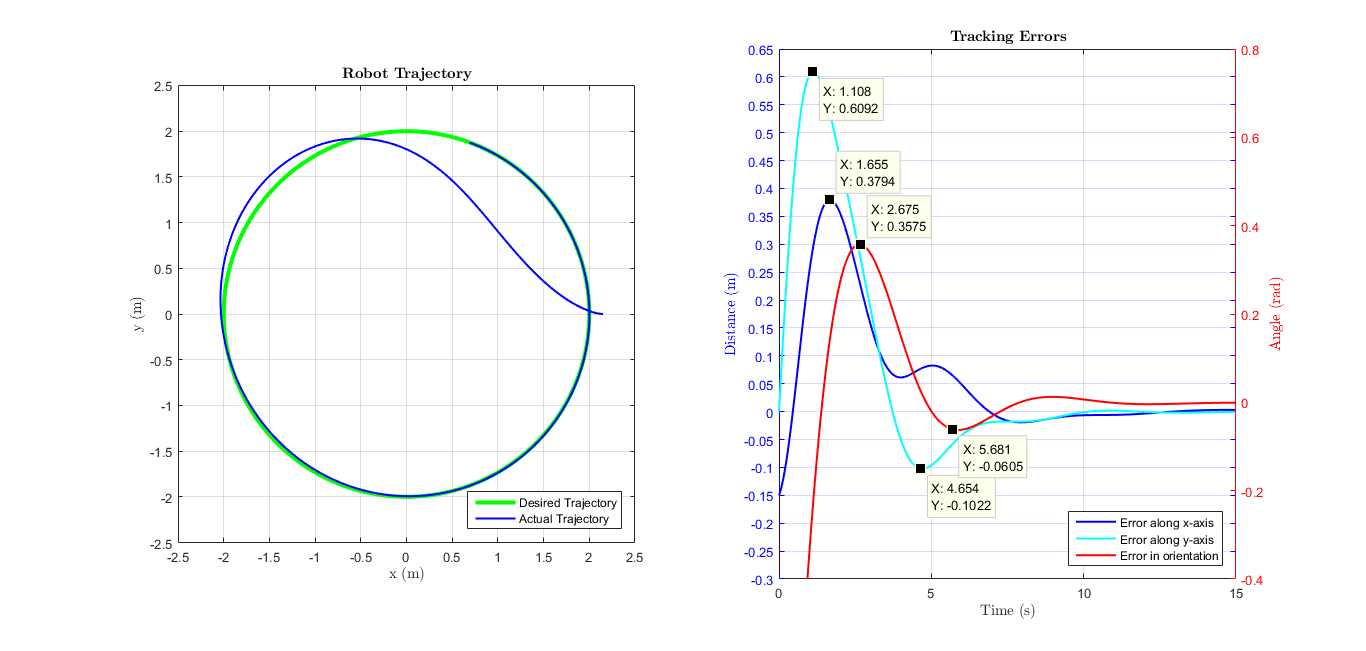
\includegraphics[width = 0.8\textwidth]{Figures/figure6.png}
\caption{Robot Trajectory and errors in $R_{0}$ frame with $K_{x}=1$, $K_{y}=1$ and $K_{\theta}=1$ }
\label{fig:figure6}
\end{figure}
It can be clearly noted in the Figure 5.5 that the trajectory is stable and converges close to the reference, but the response time is high and the gains need to be re tuned to give better dynamic performance. Increasing the gains may improve the dynamic performance.
\begin{figure}[H]
\centering
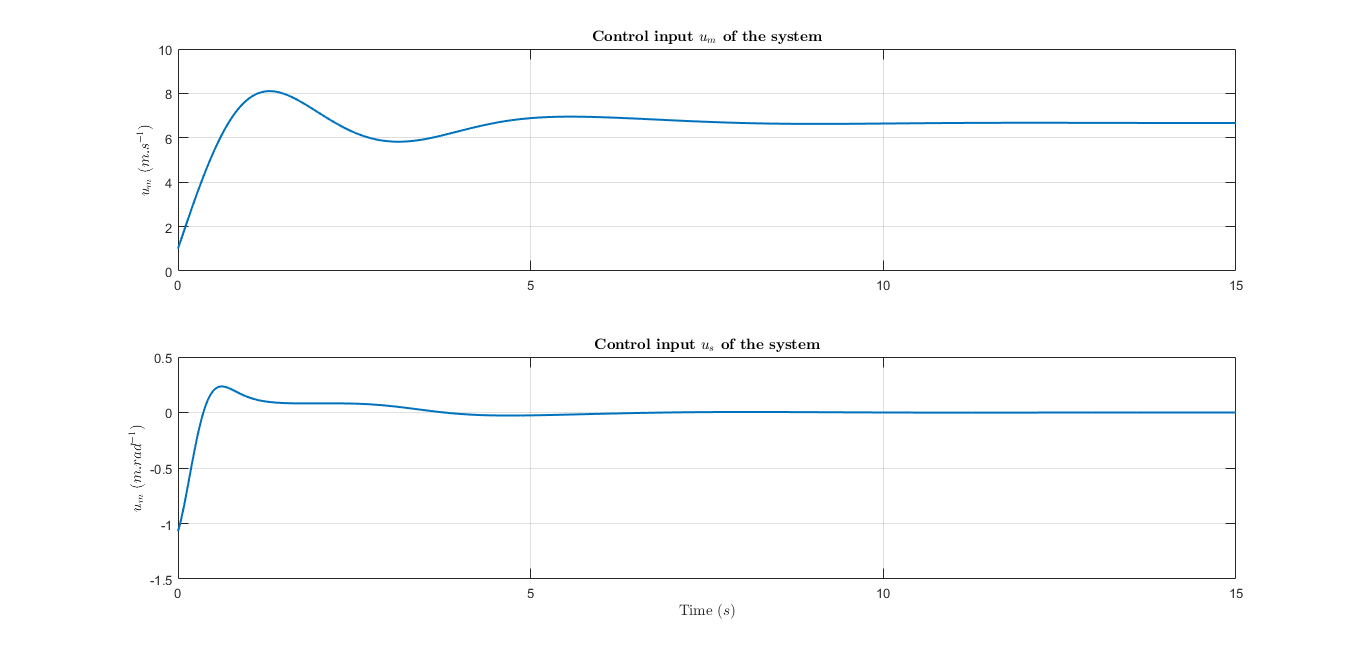
\includegraphics[width = 0.8\textwidth]{Figures/figure7.png}
\caption{The control inputs with $K_{x}=1$, $K_{y}=1$ and $K_{\theta}=1$ }
\label{fig:figure7}
\end{figure}
\item Tuning with $K_{x}=10$, $K_{y}=10$ and $K_{\theta}=10$: 
\begin{figure}[H]
\centering
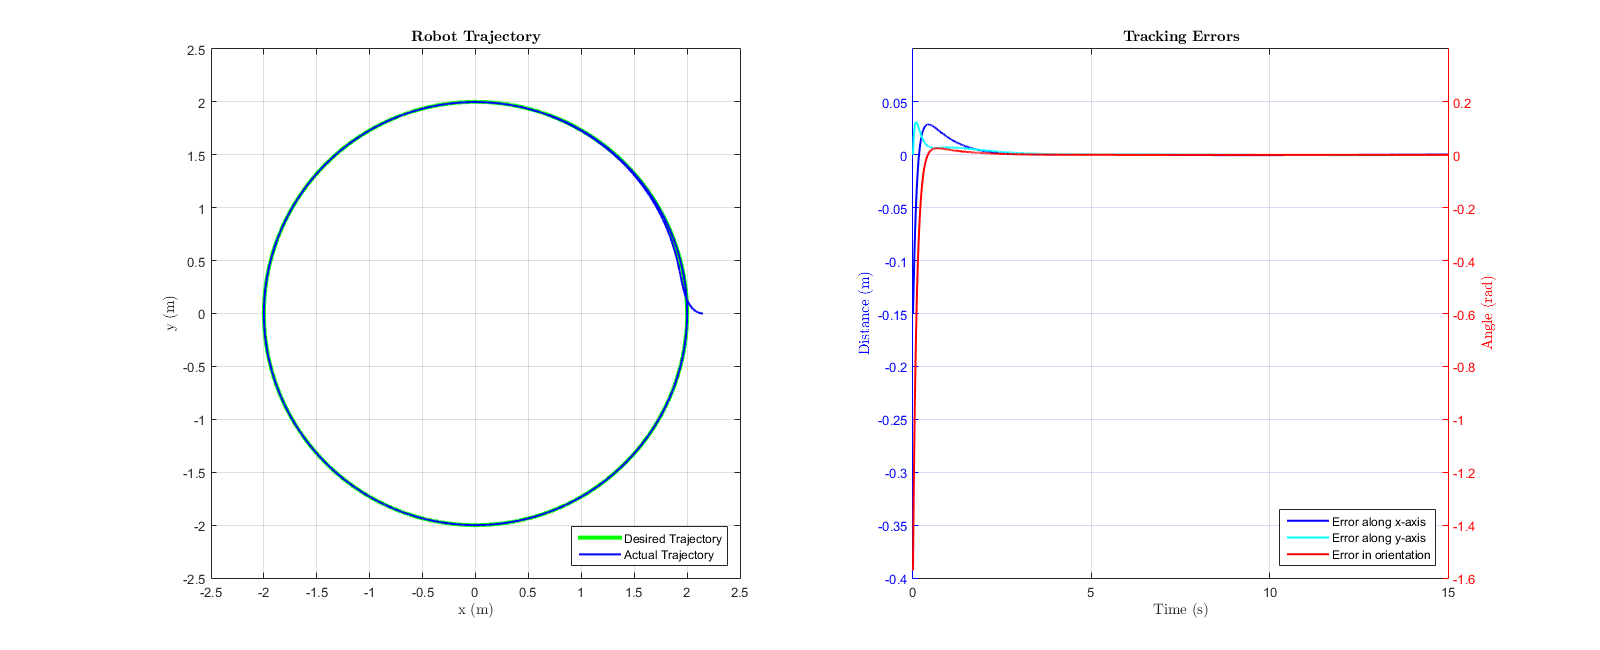
\includegraphics[width = 0.8\textwidth]{Figures/figure8.png}
\caption{Robot Trajectory and errors in $R_{0}$ frame with $K_{x}=10$, $K_{y}=10$ and $K_{\theta}=10$ }
\label{fig:figure8}
\end{figure}
As can be noted in the Figure 5.7, the dynamic performance has improved significantly and the error in $\theta$ converges to a constant value in the order of $10^{-4}$ radians but the error in $x$ and $y$ oscillate slowly about zero with a significantly low magnitude in the order of $10^{-5}$ metres. The settling time is approximately 3.5 seconds. Increasing the gains further may give better results in the simulation but practically the gain cannot be increased indefinitely as high gains can make the system unstable and saturate the actuators. 
\begin{figure}[H]
\centering
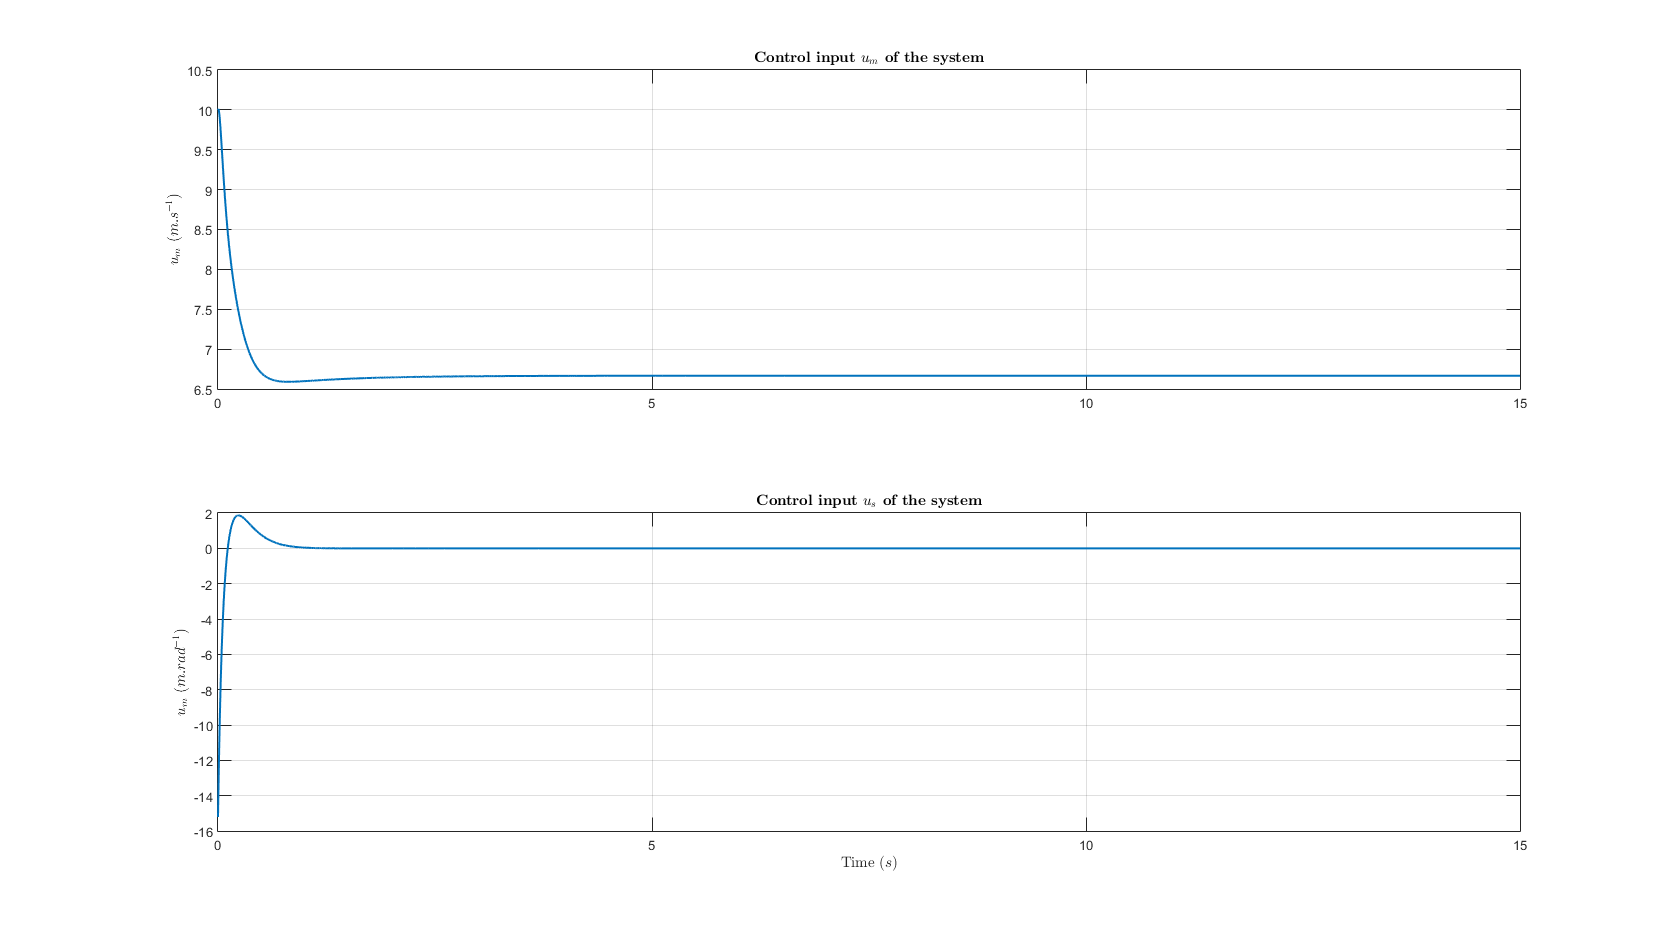
\includegraphics[width = 0.8\textwidth]{Figures/figure9.png}
\caption{Control inputs with $K_{x}=10$, $K_{y}=10$ and $K_{\theta}=10$ }
\label{fig:figure9}
\end{figure}
\end{itemize}

\textbf{Effect of Parameter Variation:}
\begin{itemize}
\item \textbf{Case 1:} 10\% increase in value of \textbf{a} only
\begin{figure}[H]
\centering
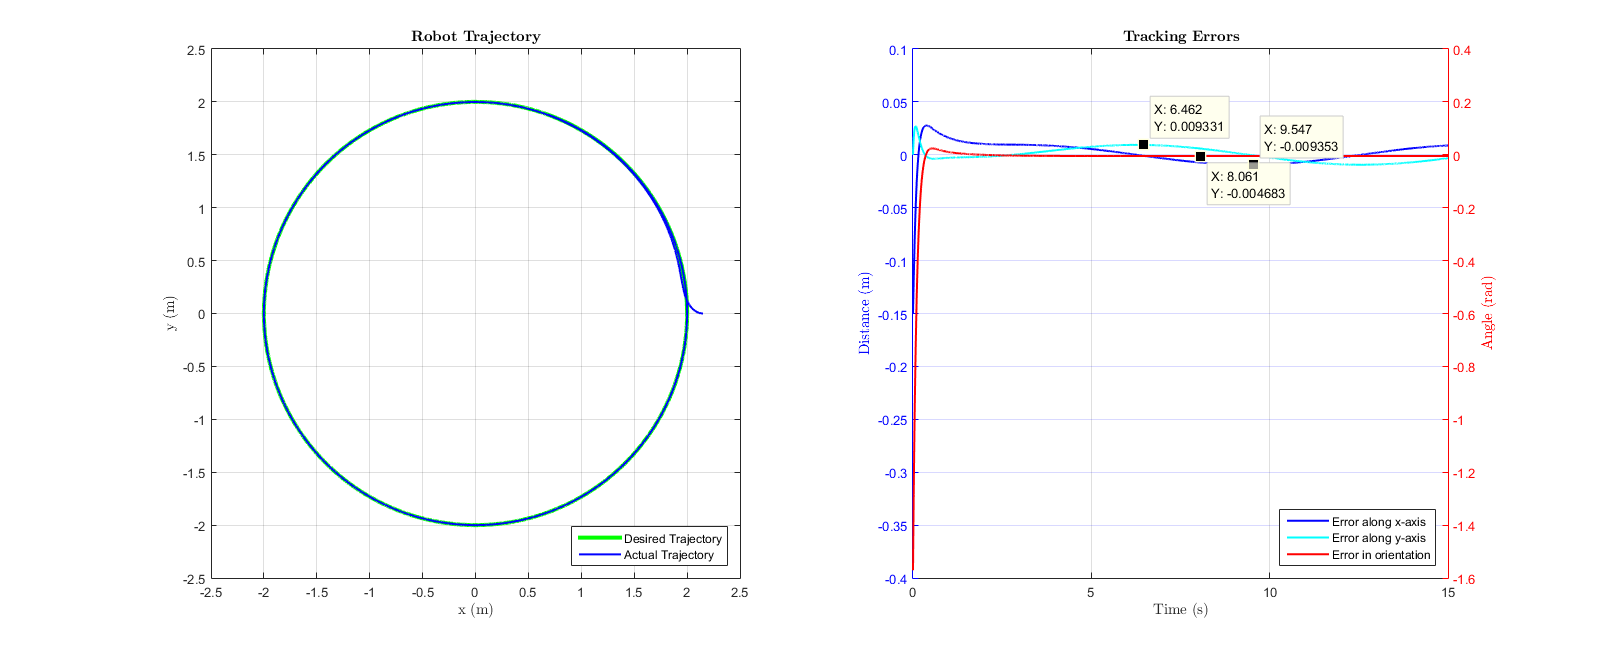
\includegraphics[width = 0.8\textwidth]{Figures/figure10.png}
\caption{ Robot Trajectory and errors in $R_{0}$ frame with $K_{x}=10$, $K_{y}=10$ and $K_{\theta}=10$ and 10\% increase in \textbf{a} }
\label{fig:figure10}
\end{figure}
The effect of parameter variation can be observed by comparing Figure 5.7 and Figure 5.9. In this case, error in $x$ and $y$ oscillate with a greater amplitude ($0.0094$ metres and $0.0093$ metres respectively )  and the error in orientation $\theta$ increases to a new steady state value ($-0.004683$ radians). The overall performance has deteriorated due to parameter variation.
\begin{figure}[H]
\centering
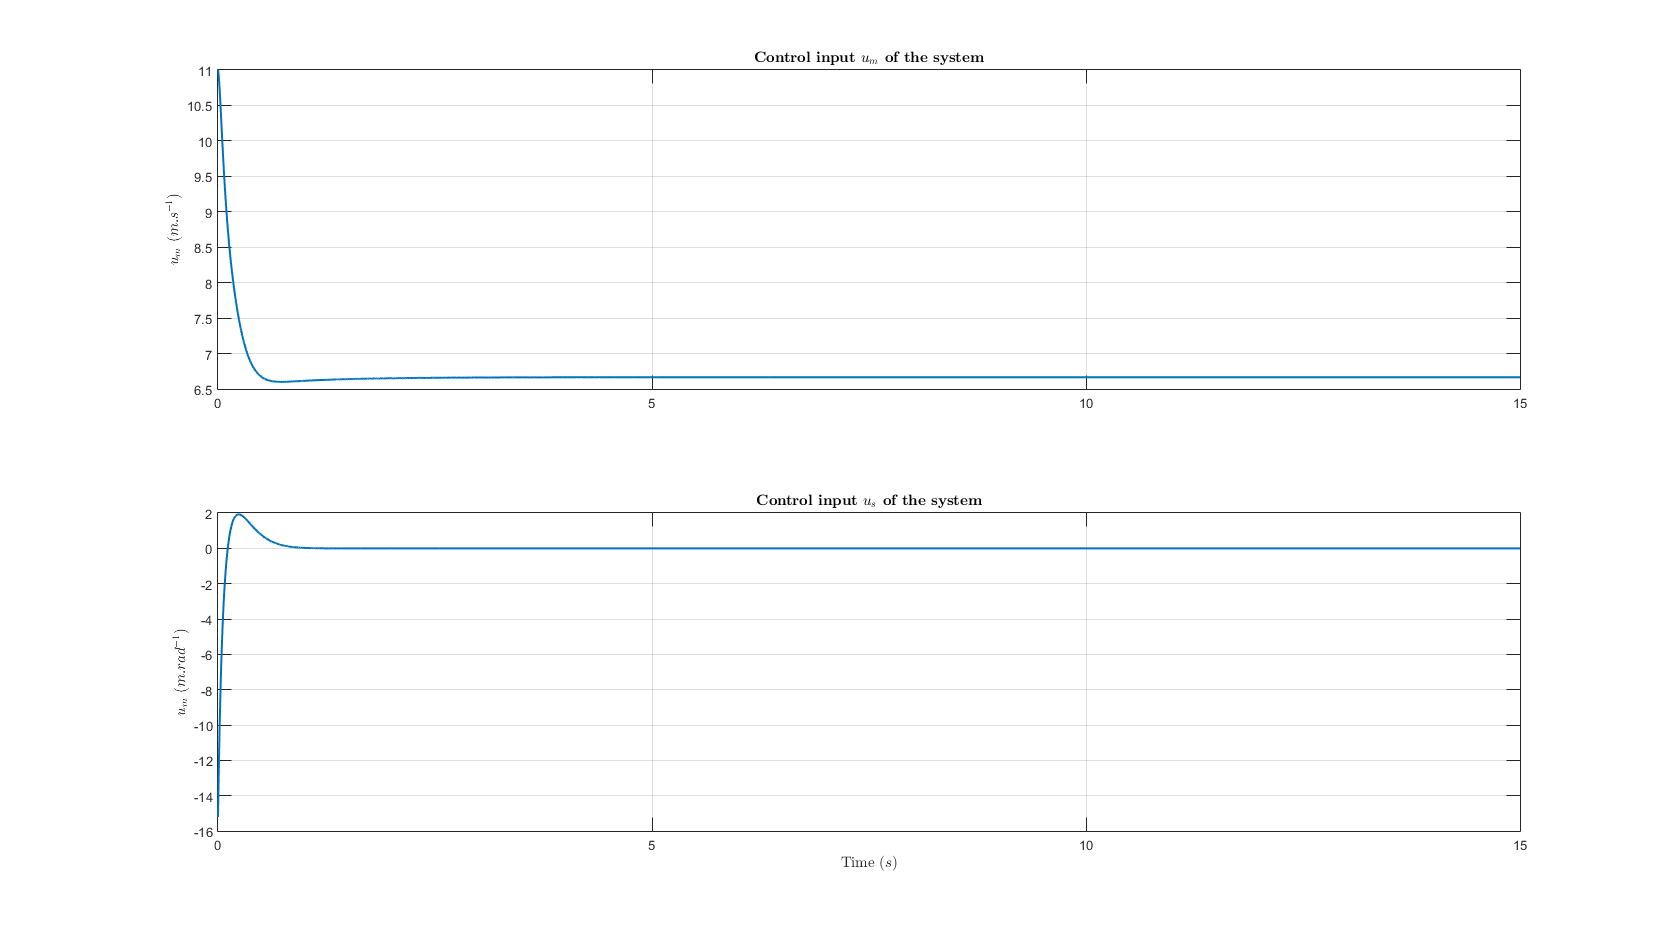
\includegraphics[width = 0.8\textwidth]{Figures/figure11.png}
\caption{ Control inputs with $K_{x}=10$, $K_{y}=10$ and $K_{\theta}=10$ and 10\% increase in \textbf{a} }
\label{fig:figure11}
\end{figure}

A possible solution to reduce the effect of parameter variation could be increasing the gains within reasonable limits. On making  $K_{x}=25$, $K_{y}=25$ and $K_{\theta}=15$, a reduction in error magnitudes can be seen (Figure 5.11). The errors in $x$ and $x$ now oscillate slowely with a lower amplitude ($0.0037$ metres in both axes) and the error in orientation $\theta$ has also reduced to a lower steadt state value ($-0.001881$ radians).

\begin{figure}[H]
\centering
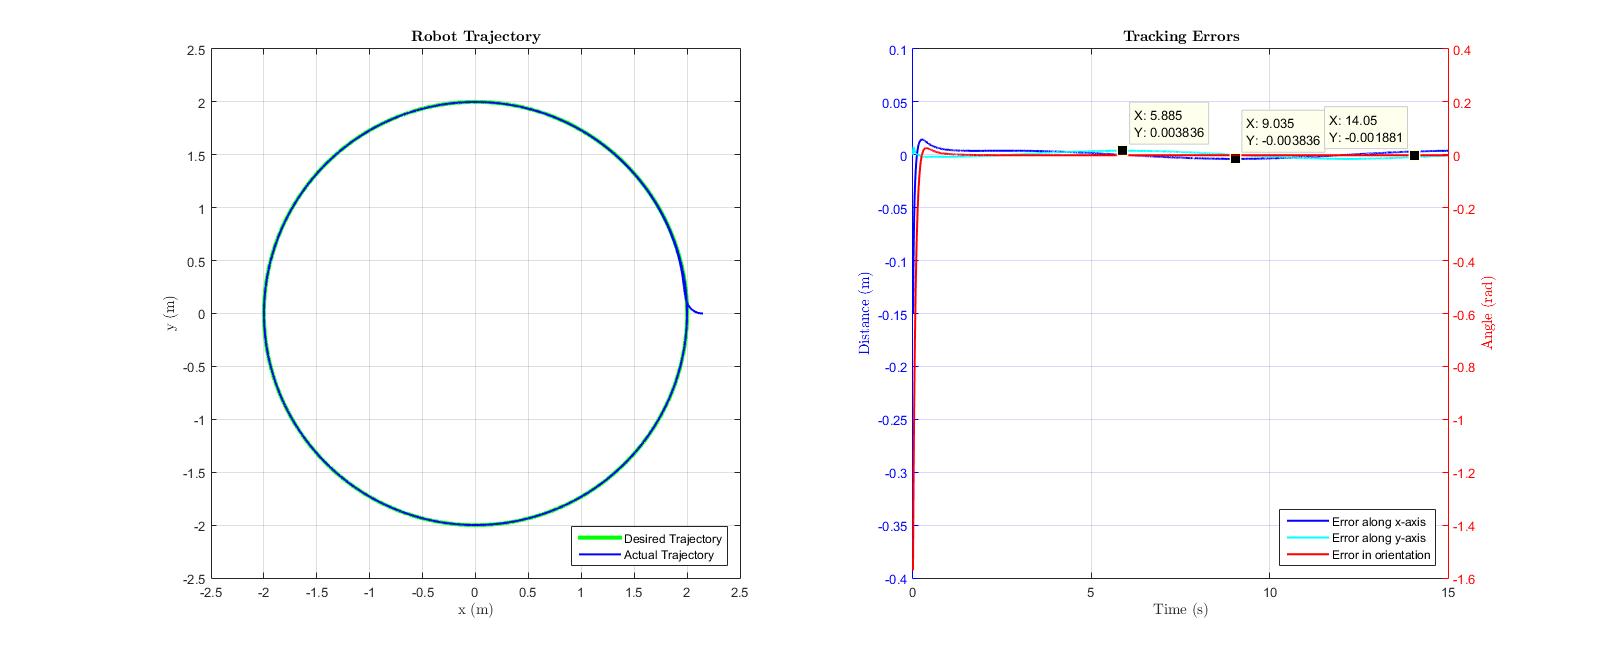
\includegraphics[width = 0.8\textwidth]{Figures/figure12.png}
\caption{  Robot Trajectory and errors in $R_{0}$ frame with $K_{x}=25$, $K_{y}=25$ and $K_{\theta}=15$ and 10\% increase in \textbf{a}  }
\label{fig:figure12}
\end{figure}

\item \textbf{Case 2:} 10\% increase in value of \textbf{r} only\\
As in Case 1, the effect of variation in \textbf{r} results in oscillatory errors in $x$ and $y$ with higher amplitude(approximately $0.009717$ metres in both axes) and increased steady state error in $\theta$ (approximately $0.004859$ radians) as shown in Figure 5.12. A higher gain tends to mitigate this problem as observed in Figure 5.14.
The errors in $x$ and $y$ reduce to a lower amplitude (approximately $0.003978$ metres in both axes) and converge to a reduced steady state error in $\theta$ (approximately $0.001952$ radians).
\begin{figure}[H]
\centering
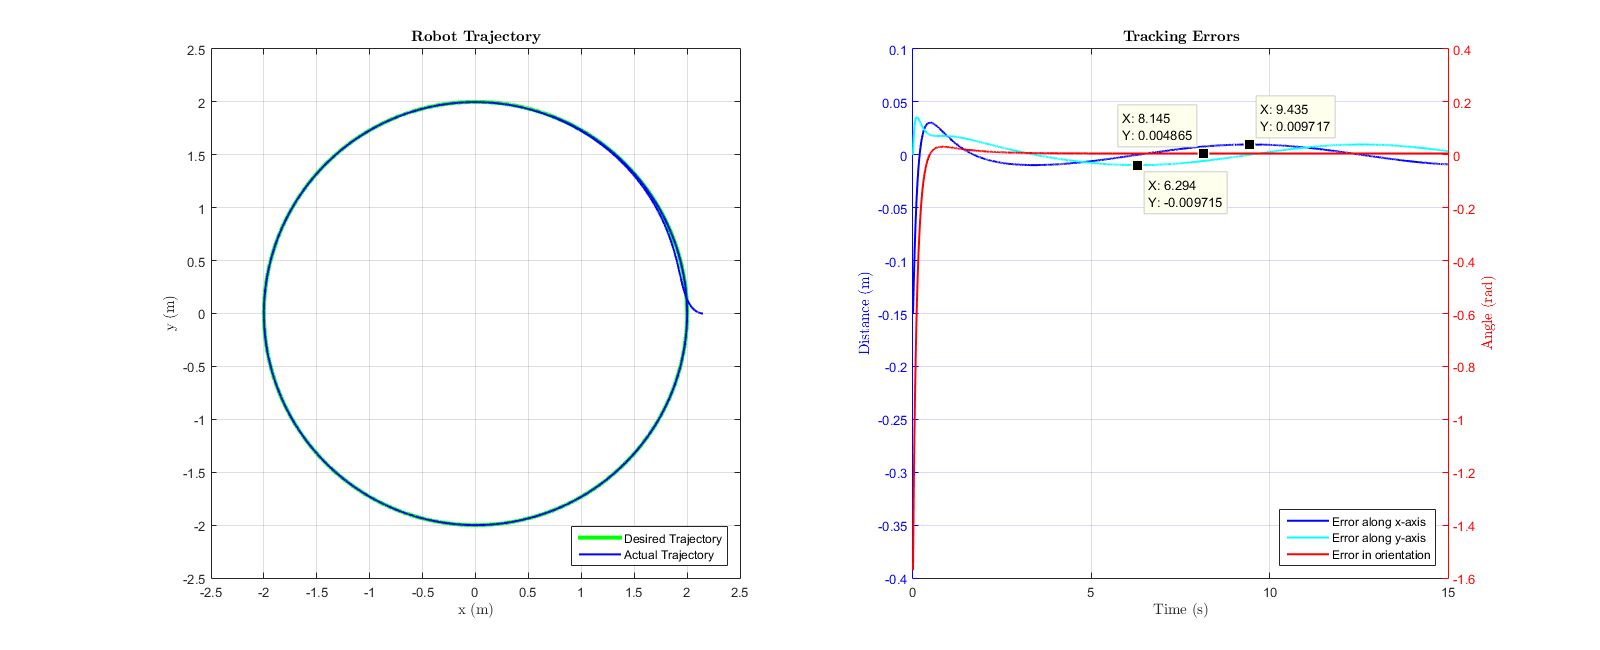
\includegraphics[width = 0.8\textwidth]{Figures/figure14.png}
\caption{ Robot Trajectory and errors in $R_{0}$ frame with $K_{x}=10$, $K_{y}=10$ and $K_{\theta}=10$ and 10\% increase in \textbf{r} }
\label{fig:figure13}
\end{figure}
\begin{figure}[H]
\centering
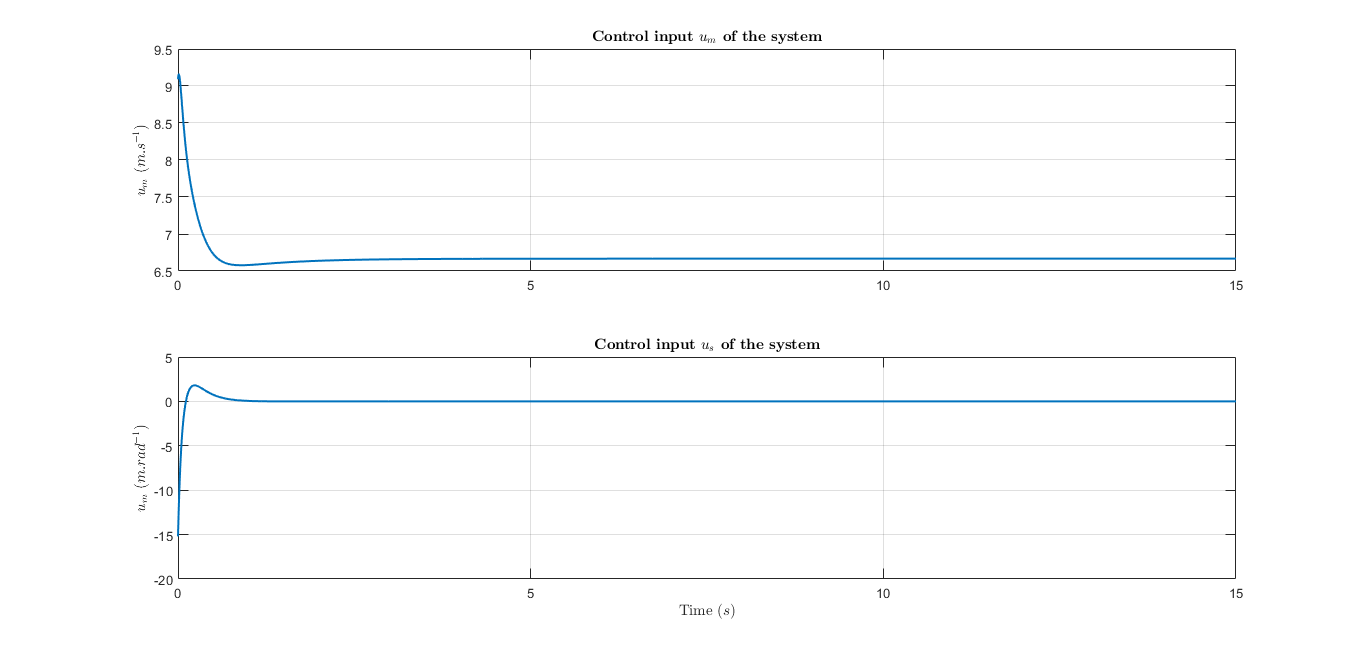
\includegraphics[width = 0.8\textwidth]{Figures/figure15.png}
\caption{ Control inputs with $K_{x}=10$, $K_{y}=10$ and $K_{\theta}=10$ and 10\% increase in \textbf{r} }
\label{fig:figure14}
\end{figure}
\end{itemize}

\begin{figure}[H]
\centering
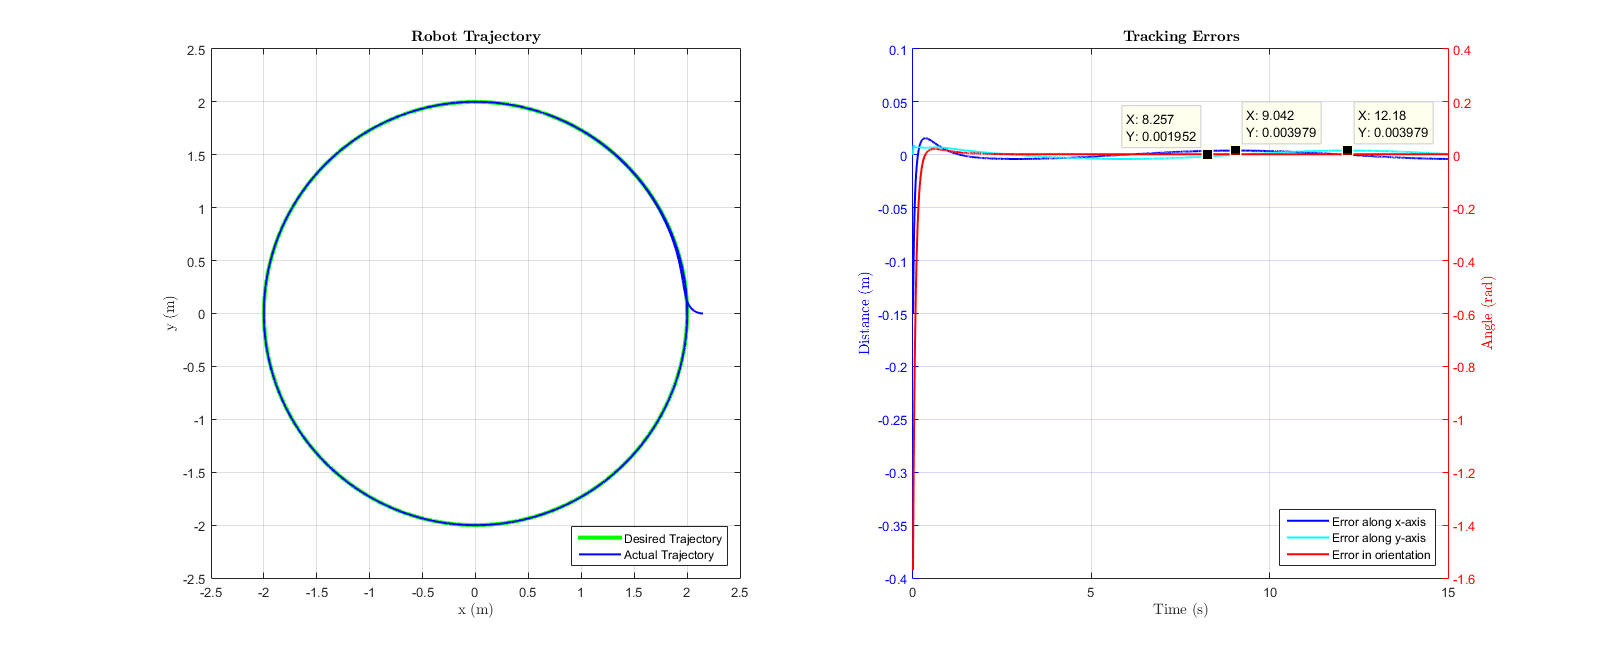
\includegraphics[width = 0.8\textwidth]{Figures/figure16.png}
\caption{  Robot Trajectory and errors in $R_{0}$ frame with $K_{x}=25$, $K_{y}=25$ and $K_{\theta}=15$ and 10\% increase in \textbf{r}  }
\label{fig:figure15}
\end{figure}
The effect of 10\% decrease in the above parameters gives similar results but with changes in magnitude and phases, nevertheless, the errors reduced when a higher gains are applied.
\end{document}